\documentclass{standalone}

\usepackage{tikz}

\begin{document}
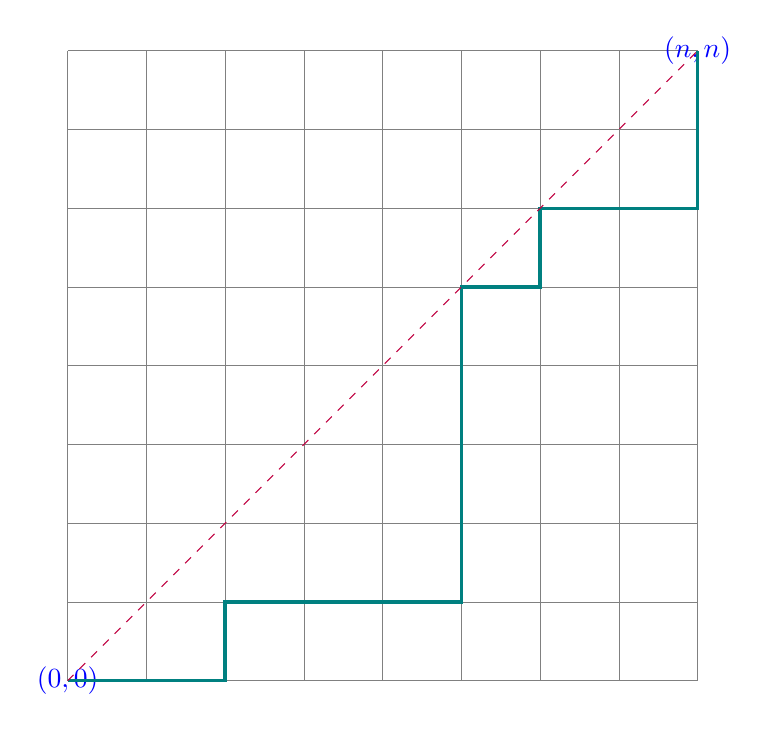
\begin{tikzpicture}
  \draw[help lines] (0,0) grid (8,8);

  \node (00) [blue] {$(0,0)$};
  \node (nn) [blue] at (8,8) {$(n,n)$};

  \draw[teal, very thick] (0,0) -- (1,0) -- (2,0) 
    -- (2,1) -- (3,1) -- (4,1) -- (5,1) 
    -- (5,2) -- (5,3) -- (5,4) -- (5,5)
    -- (6,5) -- (6,6)
    -- (7,6) -- (8,6)
    -- (8,7) -- (8,8);

  \draw[purple, dashed] (00.center) to (nn.center);
\end{tikzpicture}
\end{document}
